\documentclass{cshonours}
\bibliographystyle{acm}

\usepackage{graphics}  %optional
\usepackage{amsmath}
\usepackage{algorithm,algorithmicx,algpseudocode}
\usepackage[scientific-notation=true]{siunitx}

\title{RNA Folding: Beyond the Thermodynamic Hypothesis}
\author{Max Ward (20748588)}

\keywords{Ribonucleic acid, secondary structure, prediction}
\categories{J.3 Biology and genetics}

\begin{document}
\maketitle

\begin{abstract}
Algorithmic prediction of Ribonucleic Acid (RNA) secondary structure has been actively researched since the 1970s. RNA is a biologically active molecule with many poorly understood functions. For example, it is involved in regulation of DNA expression, has been implicated in developmental pathways, and acts as a catalyst for many biological processes. Quick and accurate prediction of RNA structure is therefore essential for further elucidation of its role. The Thermodynamic Hypothesis, which is the fundamental dogma underlying protein folding algorithms, has been applied successfully to the RNA folding problem. Unfortunately, this success is only partial; RNA folding algorithms are currently not able to reliably predict correct structures. These algorithms typically globally optimize some scoring function, usually thermodynamic stability. This is in keeping with the Thermodynamic Hypothesis. However, there is evidence that some RNAs fold into suboptimal states. One possible explanation is kinetic folding, which posits that structures form during transcription. In this investigation I hypothesize that local interactions are stronger than global interactions during RNA structure formation. To test this, a sliding window was used to generate locally optimal structures, then various algorithms were devised to merge these structures. An array of window sizes was tried, and the best were recorded. Given the right window size, the resulting predictions were more accurate than corresponding globally optimal structures, using the same model of RNA folding. I argue that this constitutes strong support for my hypothesis. In addition, a new algorithm called `$ab$-splat', which was based on the computation of locally optimal windows, is introduced. This algorithm, while  naive, had comparable prediction accuracy to the RNAfold algorithm, which is part of the ViennaRNA suite. Additionally, it runs an order of magnitude faster, and uses less memory.
\end{abstract}


\tableofcontents
\listoftables  %optional
\listoffigures  %optional



\chapter{Introduction}

A widely held axiom is that chemical structure is tantamount to biological function. Because Ribonucleic acid (RNA) is at the core of many biological processes, it is essential to accurately predict its structure. Furthermore, this will allow the detection and classification of unknown RNAs, and assist the design of new RNA based drugs \cite{condon2003problems}.

The most general RNA secondary structure prediction algorithms are those that do so de novo. This is with only the primary sequence, and no auxiliary information. These algorithms typically minimize the free energy of folded RNA secondary structures. This bias is largely due to the `Thermodynamic Hypothesis'. Anfinsen \cite{anfinsen1973principles} presented this hypothesis as the underlying principle for the formation of biologically active proteins. He held that proteins fold into a minimum Gibbs free energy conformation in their typical biological environment. This insight has been invaluable for folding proteins and RNAs in silico. Despite this, methods for the prediction of RNA secondary structures have hit an upper limit in accuracy. One explanation for this is kinetic folding, a paradigm in which the physical process of RNA transcription can prevent global minimisation of free energy.

Kinetic folding has been observed in vivo, and evidence has existed since the early 80s. Kramer and Mills \cite{kramer1981secondary} reported seeing preliminary secondary structures form, break apart, and reform into other structures during transcription. This means that as RNA is synthesized its structure is already undergoing dynamic formation with every additional nucleotide. Over a decade later, Morgan and Higgs \cite{morgan1996evidence} examined many RNA molecules and found that typical structures have suboptimal free energy. They postulated that this is due to kinetic folding, and that errors in the free energy parameters of the current model cannot fully explain the discrepancy. Recently, Proctor and Meyer \cite{proctor2013cofold} improved secondary structure prediction accuracy by simulating kinetic folding. In their method, the effects of kinetic folding are captured using a scaling function in which closer nucleotides are weighted higher than distant nucleotides. Proctor and Meyer \cite{proctor2013cofold} reported that this improves prediction accuracy; particularly for RNA molecules comprising greater than 1000 nucleotides. 

I propose that, in RNA molecules, local interactions are stronger than global interactions. As a result, RNA molecules will fold into a global structure made up of locally optimal structures. In other words, short range interactions will predominate long range interactions. This is my core hypothesis. If this assumption is correct, it follows that there exists a set of `windows' that, when folded using any reasonable model, will be more accurate than the corresponding global optimum using the same model.

\section{Relevant Algorithms}
The most widely used de novo RNA secondary structure prediction algorithm is that of Zuker \& Stiegler [ref]. It uses dynamic programming to efficiently exploit RNA's nested structure. It can predict RNA secondary structures using only $O(n^3)$ time and $O(n^2)$ where $n$ is the number of nucleotides, and uses an experimentally determined set of thermodynamic parameters for scoring. Because of its efficiency, robustness, and extensibility, this method is, even today, still the most popular available. The most widely used packages for
RNA structure prediction all contain implementations of the Zuker-Stiegler algorithm [refs].

\begin{figure}
\begin{center}
\scalebox{0.3}{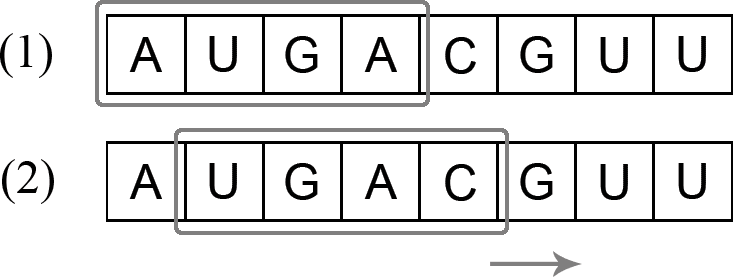
\includegraphics{slidingwindow}}
\end{center}
\caption{Depiction of how sliding windows can explore a RNA sequence.}
\label{fig:slidingwindow}
\end{figure}

This algorithm can also be efficiently used for predicting the structure of consecutive sliding windows. Naively this can be done by running a typical cubic time implementation of the Zuker algorithm at every window location. Let $L$ be defined as the chosen
window size, and $N$ represent the length of the RNA seqeucne. This leads to a total complexity of $O(NL^3)$. In 2004, Hofacker, Priwitzer, and Stadler \cite{hofacker2004prediction} lowered this bound to $O(NL^2)$. This is achieved by modifying the Zuker algorithm. Specifically, the dynamic programming table from the previous step is used to quickly fill the table for
the next window in quadratic time; because consecutive windows overlap, preceding information can be meaningfully used in each forward computational step.
As a result it requires only a single table of size $O(L^2)$, and as such its memory complexity is only $O(N + L^2)$.



\section{Locally Optimal Algorithms}
The following algorithms and techniques comprise our core contribution, and are based on sliding window RNA folding algorithms. Such an algorithm generates a set of consecutive locally optimal windows. I shall now precisely define how these windows were processed, and how they can be used to predict a full RNA secondary structure.

\subsection{RNA Intervals}
Running an algorithm which generates consecutive windows of size $L$ over a RNA primary sequence of size $n$ produces $n-L+1$ windows of size $L$. Each of these windows contains the optimal secondary structure for that subsequence of RNA. This structure is computed with complete disregard for any interactions outside the bases encompassed by the window. It is therefore locally optimal, but not globally optimal. The secondary structure may contain no bonds at all, or it might contain an elaborate structure. Such a structure might have disjoint components. An example of this is shown in Figure \ref{fig:rnainterval}, in which there are two distinct substructures which are part of no larger substructure. A substructure is disjoint if and only if no bond encompasses it and another substructure.

I extracted all disjoint substructures from the structures computed by the sliding window algorithm. I called these `RNA intervals'. This was done so that structures from different windows could be effectively blended. Every RNA interval was assigned a score. This score was defined as the amount of free energy reduction which that RNA interval contributes. Figure \ref{fig:rnainterval} contains a diagrammatic representation of both the sliding window, and the RNA intervals it comprises. In the diagram, only a single window is shown, however the same logic holds for all previous and subsequent windows. RNA structure is represented using dot-bracket notation. In this style, every matching pair of parentheses represents bonded base pairs. Conversely, a full stop represents an unbonded base. In the figure, curly braces indicate the ends of windows and RNA intervals. The computed structure for the window contains two disjoint substructures, these are split into two RNA intervals. These are disjoint because they are contained within no other bond. The RNA interval merging algorithms, which I shall now discuss, worked on these disjoint substructures, rather than on the entire structures produced by the sliding window.


\begin{figure}
\begin{center}
\scalebox{0.35}{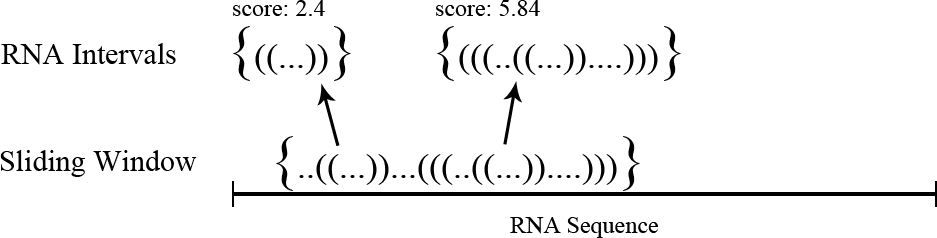
\includegraphics{rnainterval}}
\end{center}
\caption{The relationship between a sliding window and its RNA intervals. RNA secondary structures are represented using dot-bracket notation.}
\label{fig:rnainterval}
\end{figure}




\subsection{Merging RNA Intervals}
\label{sec:merging}

Given a RNA sequence, one can generate a set of RNA intervals by running any sliding window algorithm, and storing the RNA intervals generated for each window location. Many of these intervals will overlap, or contain fragments of one-another. To construct a plausible and complete secondary structure for the original RNA, a subset of the RNA intervals generated this way must be selected. I tried several methods for doing this. The goal of such an algorithm is to produce a valid secondary structure out of a set of RNA intervals which is as accurate (compared to the actual secondary structure) as possible.

\begin{figure}
\begin{center}
\scalebox{0.35}{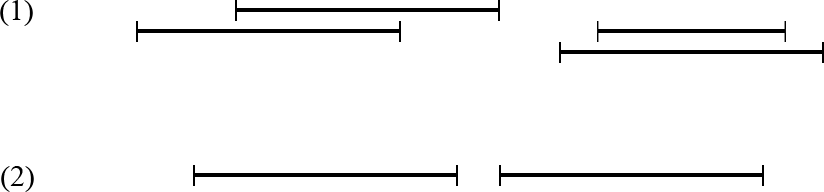
\includegraphics{compat}}
\end{center}
\caption{Case 1 shows RNA intervals that are not compatible. Case 2 shows an example of compatible intervals.}
\label{fig:compatible}
\end{figure}



\subsubsection{Weighted Activity Selection}
The best method for merging RNA intervals was Weighted Activity Selection (WAS). The WAS problem is a generalization of the activity selection problem. Given a set of intervals, each of which is assigned a weight, the problem is to find a subset such that none of these intervals touch one-another, and the sum of their weights is maximised. This can be solved in $O(n \log n)$ time and using $O(n)$ space. It maps naturally to the problem domain of this investigation. I used this algorithm to find the subset of compatible windows which have the minimum sum free energy.



\subsection{Prediction Using Windows}
\label{sec:absplat}
RNA interval merging algorithms are not able to make good predictions in isolation. Hence, an approach was devised to predict RNA secondary structures using them. In this approach I computed sliding windows for a set of sizes---a sample like this is often called a `splat'. Weighted Activity Selection was then done on the resulting set of computed RNA intervals.  This was because it appeared to be the best RNA interval merging algorithm, see Section \ref{sec:localopt} for details. I explored several methods for finding good splats. I present here the most successful technique, which I call `$ab$-splat' prediction. Initially the algorithm starts at a small window size, and exponentially increases the scope of the window until a threshold is exceeded. This is explained using pseudocode in Algorithm \ref{absplat}.

\begin{algorithm}
  \caption{$ab$-splat}
  \label{absplat}
  \begin{algorithmic}[1]
  \State Let $RNA$ be the primary RNA sequence being folded
  \State Let $i = a$
  \State Let $S = \{\}$
  \While{$i \leq $ \Call{Treshold}{$RNA$} }
  	\State $S = S \: \cup $ \Call{ComputeSlidingWindow}{$RNA$, $i$}
  	\State $i = i \times b$
  \EndWhile
  \State \Return \Call{WeightedActivitySelection}{$S$}
  \end{algorithmic}
\end{algorithm}

The \texttt{Threshold} function was defined as $\sqrt{ \texttt{RNA Length} } \times 9.5$. This formula was found using empirical experimentation. In addition, $a$ and $b$ are arbitrary constants set by the user. I shall discuss how I found good values for them in Section \ref{sec:absplatmethod}. The \texttt{ComputeSlidingWindow} function was a modified implementation of Hofacker, Priwitzer, and Stadler's \cite{hofacker2004prediction} algorithm, described in Section \ref{sec:localopt}. It first computes all consecutive windows for a fixed size $i$, breaks these up into RNA intervals, and returns the set of these RNA intervals.

\subsubsection{Time Complexity}

The time complexity of this algorithm is non-trivial to deduce. The runtime of \texttt{ComputeSlidingWindow} is $O(nL^2)$ where $L$ is the window size, and $n$ is the length of the RNA. It is called once for every window size. In addition \texttt{WeightedActivitySelection} uses $O(n \log n)$ time, where $n$ is the number of RNA intervals in the set $S$. I shall now show that $ab$-splat has a worst case time complexity of $O(n^2)$.

The sequence of window sizes explored by $ab$-splat given any values for $a$ and $b$ are as follows.

\begin{equation} \label{eq:windowsizes}
	ab^0, \; ab^1, \; ab^2, \; ab^3 \; \cdots ab^{\log_b \sqrt{n}-1}
\end{equation}

This sequence is of course bounded by the \texttt{Treshold} function which means that all terms are $O(\sqrt{n})$. It follows that there are $O(\log_b \sqrt{n})$ terms in the series.  Geometric progressions of this type have the following identity.


\begin{equation}
	ab^0 +  ab^1 +  ab^2 +  ab^3 +  \cdots + ab^{n-1} = \frac{a(1-b^n)}{1-b}
\end{equation}

Which means that the closed form of Equation \ref{eq:windowsizes} is as follows.

\begin{equation}
  \frac{a(1-b^{\log_b \sqrt{n}})}{1-b}
\end{equation}

Since $a$ and $b$ are both constant values, this is $O(\sqrt{n})$. Thus, the sum of all window sizes as defined in Equation \ref{eq:windowsizes} is $O(\sqrt{n})$. \texttt{ComputeSlidingWindow} is run for every window size defined in this sequence. Since the time complexity of \texttt{ComputeSlidingWindow} is $O(nL^2)$, and the sum of all window sizes is $O(\sqrt{n})$, the cumulative work is $O(n(\sqrt{n})^2)$ which trivially simplifies to $O(n^2)$. Now I shall show that this dominates the cost of running Weighted Activity Selection.

Every window size produces $O(n)$ windows of size $L$. Every such window can contain at most $O(L)$ RNA intervals. Because the sum of all windows sizes is $O(\sqrt{n})$, and we collect $O(n)$ sets of windows, we are left with an upper bound of $O(n^\frac{3}{2})$ RNA intervals in total.


Weighted Activity Selection uses $O(n \log n)$ time. As we have $O(n^\frac{3}{2})$ RNA intervals in the worst case, this leads to a worst case time complexity of $O(n^\frac{3}{2} \log n)$, which is dominated by $O(n^2)$. Computing the largest sliding window requires only $O(n)$ space, since it uses $O(L^2)$ space in all cases, and the largest window size is $O(\sqrt{n})$. Weighted Activity Selection additionally requires only $O(n^\frac{3}{2})$ space. As all of these RNA intervals must be stored in $S$, $ab$-splat will thus use $O(n^\frac{3}{2})$ memory in the worst case. In contrast, the Zuker algorithm requires $O(n^3)$ time and $O(n^2)$ space. The computational bottleneck is usually time, however. 


\chapter{Results}
\section{Interval Selection}
The purpose of the following tests was to determine if any RNA interval merging algorithms (see Section \ref{sec:merging}) could potentially achieve better accuracy than globally optimizing algorithms. The RNAfold package is a modern implementation of the Zuker algorithm, which globally optimizes a thermodynamic scoring scheme. RNAfold is thus used for comparison. I predicted that some merging algorithms should have higher accuracy if local interactions are stronger than global interactions during RNA folding.

The average score between all RNA interval selection algorithms was compared (see Table \ref{tab:summaryselection}). The highest scoring algorithm appeared to be Top-Down Selection, closely followed by Weighted Activity Selection, then by Bottom-Up Selection. To verify this performance gap, a Wilcoxon Signed-Rank test was done to compare the recorded F-scores for corresponding RNA. This test was chosen because the data recorded did not appear to be parametric. While this test reflected the small difference in averages between Weighted Activity Selection and Top-Down Selection ($z = 1.33066$, see Table \ref{tab:wilcoxonselection}), it was not statistically significant ($p > 0.05$). To further test Top-Down Selection and Weighted Activity Selection, another Wilcoxon Signed-Rank test was done on only RNAs of length $\geq 300$ bases. This revealed a moderate but statistically significant difference, indicating that Weighted Activity Selection generally had higher F-scores for larger RNAs ($p < 0.001, z = 4.55591$). Finally, a Wilcoxon Signed-Rank test was done between Weighted Activity Selection and Score Selection to check for circular dominance. In accordance with the mean F-score values, Weighted Activity Selection appeared to have higher F-scores than Score Selection ($p < 0.001, z = 12.0957$).

\begin{table}
\centering
\begin{tabular}{l*{6}{c}r}
Algorithm	& Mean & Median \\
\hline
BUS &  0.38122    &    0.35065   \\
SS & 0.68373    &    0.73098  \\
WAS & 0.70395   &     0.75709  \\
TDS & 0.71684   &     0.80000  \\
\hline
RNAfold & 0.57483    &    0.60870 \\
\end{tabular}

\caption{Summary statistics of recorded F-scores for Weighted Activity Selection (WAS), Top-Down Selection (TDS), Bottom-Up Selection (BUS), Score Selection (SS), and RNAfold.}
\label{tab:summaryselection}
\end{table}



A Wilcoxon Signed-Rank test was also used to compare the best recorded F-scores for all RNA interval selection algorithms, and those recorded for RNAfold (see Table \ref{tab:wilcoxonselection}). All tests were statistically significant ($p < 0.001$). All algorithms but Bottom-Up Selection were shown to outperform RNAfold; Weighted Activity Selection in particular ($z = 13.2082$). Figure \ref{fig:wasrnafold} clearly depicts this performance difference.


\begin{table}
\centering
\begin{tabular}{l*{6}{c}r}
Test Subjects	& $z$-value & Two-tailed $p$-value \\
\hline
WAS \& TDS 	& -1.33066 &	0.183301 \\
WAS \& TDS (RNA length $\geq 300$)	& 4.55591 &	$2.60801 \times 10 ^{-6}$ \\
WAS \& SS & 5.94681 &	$2.73418 \times 10^{-9}$  \\
\hline
BUS \& RNAfold & -9.13933 &	$6.28392 \times 10^{-20}$  \\
SS \& RNAfold & 12.0957 &	0  \\
TDS \& RNAfold & 13.119 &	0  \\
WAS \& RNAfold & 13.2082 &	0  \\
\end{tabular}

\caption{Results of Wilcoxon Signed-Rank testing for F-scores. Weighted Activity Selection (WAS), Top-Down Selection (TDS), Bottom-Up Selection (BUS), Score Selection (SS), and RNAfold are included.}
\label{tab:wilcoxonselection}
\end{table}


\begin{figure}
\begin{center}
\scalebox{1}{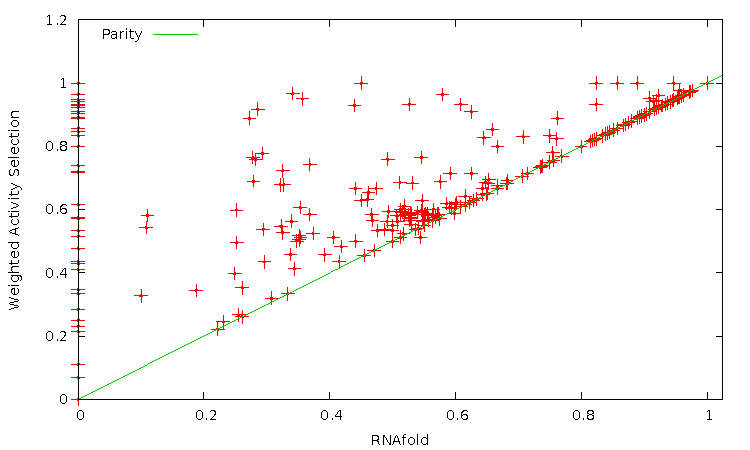
\includegraphics{wasrnafoldplot}}
\end{center}
\caption{F-scores for matching RNA test cases achieved by Weighted Activity Selection and RNAfold plotted against one-another. The green line represents parity. Any points above the line are cases in which Weighted Activity Selection performed better; points below the line indicate that RNAfold was more accurate. Note that a maximum F-score is \texttt{1.0}.}
\label{fig:wasrnafold}
\end{figure}


\section{RNA Intervals For Prediction}
\label{sec:res_absplat}
The purpose of the following tests was to determine if the $ab$-splat algorithm (see Section \ref{sec:absplat}) was more accurate than RNAfold. Additionally, further tests were undertaken to compare the runtime efficiency of both algorithms. It was expected that $ab$-splat would be more accurate than, and run faster than, RNAfold.

An Ordinary Least Squares linear regression was done to determine the correlation between F-scores recorded for $ab$-splat in the training and validation sets. Figure \ref{fig:abcorrelation} depicts the resulting model. A strong correlation was found ($R^2 = 0.703$, $p < 0.001$) for scores in the training set versus scores in the validation set. The best $ab$ value pair found in the training set was $a = 24$, $b = 1.8$. The $ab$-splat algorithm was configured using these values. As the data did not appear to be normally distributed, a Wilcoxon Signed-Rank test was done to compare F-scores for $ab$-splat (with the best $ab$ pair) and RNAfold. This test revealed a small difference in the F-scores in the population ($z = 0.1067$), which reflected the slight difference in averages (mean RNAfold score = $0.57483$, $ab$-splat = $0.58588$). However, this discrepancy was not statistically significant ($p > 0.05$).


\begin{figure}
\begin{center}
\scalebox{1}{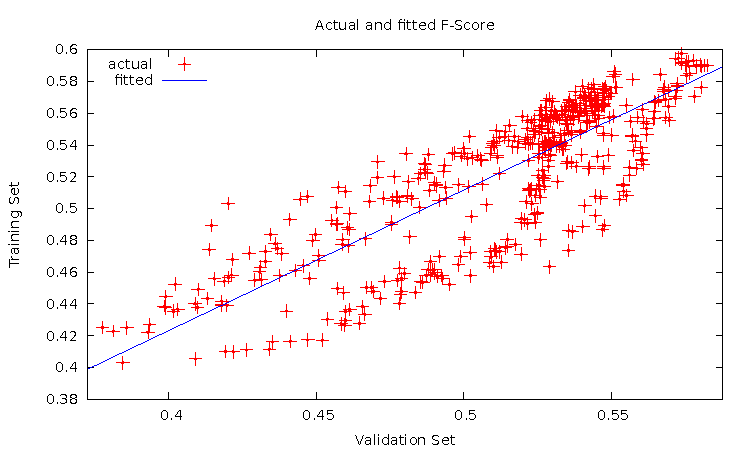
\includegraphics{abcorrelation}}
\end{center}
\caption{Correlation of F-scores for $ab$-splat in training set versus validation set. R-squared value = 0.702901, $p$-value $< 0.0001$. Standard Error of Regression = 0.025032.}
\label{fig:abcorrelation}
\end{figure}



\begin{figure}
\begin{center}
\scalebox{1}{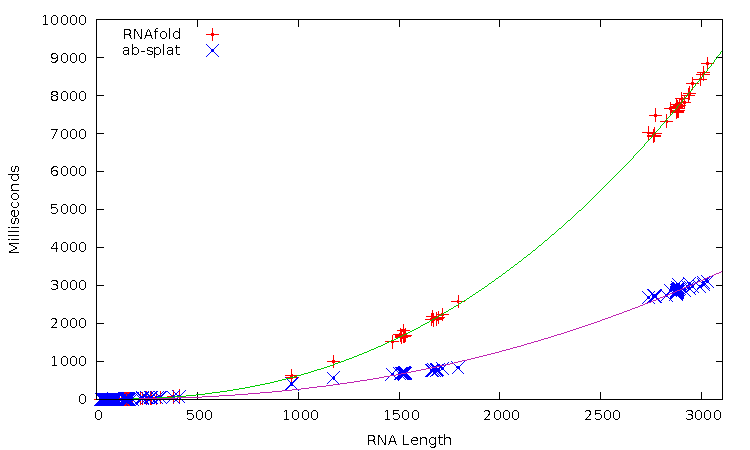
\includegraphics{zukerabtime}}
\end{center}
\caption{A comparison of the time taken for RNAfold to run against $ab$-splat. This graph indicates how much time RNAfold and $ab$-splat use with increasing RNA length. Best fit regression lines are also shown.}
\label{fig:zukerabtime}
\end{figure}

Empirical observation was used to compare the runtime of RNAfold and $ab$-splat. A graph representation of the observed times is shown in Figure \ref{fig:zukerabtime}. This graph shows how the runtime of these algorithms grow with increasing RNA length. Both appeared to have a polynomial curve. Further analysis showed that both were best approximated by a polynomial regression. Both regression equations indicated a strong relationship between RNA length and algorithmic runtime ($R^2 > 0.99$). The best fit regression line for RNAfold runtime was $O(n^{2.374})$ where $n$ is RNA length. The $ab$-splat algorithm has a best fit regression line that was $O(n^{2.25})$. A summary of the regression equations can be found in Table \ref{tab:algorithmtimeregression}.


\begin{table}
\centering
\begin{tabular}{l*{6}{c}r}
Algorithm	& Regression Equation & $R^2$ value \\
\hline
RNAfold &  $y=0.358+4.7 \times 10^{-5} \times x^{2.374}$    &    0.9997    \\
$ab$-splat & $y=2.506+ 4.67\times 10 ^{-5} \times x^{2.25}$    &    0.9985  \\
\end{tabular}

\caption{Summary of best fit regression lines for RNAfold and $ab$-splat.}
\label{tab:algorithmtimeregression}
\end{table}

\chapter{Discussion \& Conclusions}

\section{Local Optimization}
\label{sec:localopt}
The results strongly indicate that there exists local windows that, when appropriately merged, are more accurate than globally optimal structures. Given the best window size to generate RNA intervals, WAS can be markedly more accurate than RNAfold, having unequivocal statistical significance ($p \ll 0.001$). The central hypothesis of this investigation is that local interactions are stronger than global interactions during RNA folding. The Zuker algorithm, upon which RNAfold is based, finds the globally optimal secondary structure for a RNA. Weighted Activity Selection built RNA secondary structures out of locally optimal sub-structures. It follows that local interactions must be stronger than global interactions for the thermodynamic model used in the ViennaRNA suite, as the locally optimizing algorithms performed much better than the globally optimizing algorithm.

It could be argued that the results only appear to show an improvement over RNAfold because the single best window size was recorded for each RNA in the testing set. To elucidate this claim further, I shall re-state the process used to compare my RNA interval merging algorithms. For each RNA in the testing set, and for each window size from five to 500, the RNA merging algorithm was run using the RNA intervals precomputed for the given window size. The window size with the single best F-score for a given RNA was recorded. If the thermodynamic hypothesis was correct, RNA structures should have the minimal free energy configuration. This means that no locally optimal window should have higher accuracy. Clearly this is not true for the free energy model used in ViennaRNA. It may then be argued that, since our current energy model is not perfect, the difference is due to chance. This is not necessarily true; many real RNAs fold into thermodynamically suboptimal states due to kinetic folding \cite{ditzler2008rugged, treiber2001beyond}. Furthermore, my results show that all RNA interval selection algorithms (excluding Bottom-Up Selection) are consistently and significantly much more accurate across the entire test set. Statistically speaking, we can reject the hypothesis that this difference is due to chance. I suggest that the strength of local interactions in RNA folding needs to be given more weight in our current models if we are to improve their predictive power.

\subsection{Future Work}

The testing procedure used was incomplete, though compelling results were found nonetheless. Notably, only single window sizes were examined. As such, only RNA intervals found for a specific window size were used in a given secondary structure. It is possible that more accurate predictions could have been made using a combinatorial mix of window sizes to generate RNA intervals. This would provide the RNA interval merging algorithms with more intervals to choose from. Clearly this prodigiously increases the search space, which is why it was not attempted in this investigation. It might be fruitful for future research to assay combinatorial blends of many different window sizes. Additionally, while Weighted Activity Selection proved effective, there may exist better RNA interval merging algorithms.

Only the energy model implemented in RNAfold and RNALfold was used in this investigation. However, the findings presented here may also hold for other models of RNA folding. This is a classical argument from analogy. Nonetheless, locally optimized structures may prove more accurate for approaches based on SCFGs, or using machine learned parameters, or both. Because all such models are commonly based on assumptions inherited from the thermodynamic hypothesis, I argue that local optimization should work for any model of RNA secondary structure formation. The algorithms I have outlined are generic in that any folding algorithm could be used to generate sequential folds for a window of fixed size. It is important to note that using a Zuker-like energy model made this extremely efficient due to the existence of excellent sliding window algorithms; this is why it was the model of choice for this investigation.

\subsection{Implications}

I have found that there exists locally optimized secondary structures for RNAs which, in the average case, are at least 22\% more accurate than the structures predicted by RNAfold. It follows directly that local interactions must be stronger than global interactions for many RNA molecules. In short, my hypothesis was strongly supported. However, it is important to consider the practical implications of this. Unfortunately, just because such a large accuracy reservoir exists, this does not mean it can be trivially used to improve existing algorithms, or to invent new algorithms. To achieve the full accuracy improvement, an oracle algorithm must somehow guess the correct window size to use for a RNA primary sequence. As I shall explain in the following section, this does not appear to be an easy task. Regardless, it should be possible to leverage this knowledge to improve existing algorithms, or to create new algorithms with superior accuracy. 

Earlier (in Section \ref{sec:softa}), I extracted a single, salient finding from the work of Rivas \cite{rivas2013four}: that all RNA prediction algorithms seem to hit an upper limit in accuracy. I also suggested an explanation for this: that, for various historical reasons, they all implicitly adhere to the Thermodynamic Hypothesis as described by Anfinsen \cite{anfinsen1973principles}. I submit that the findings presented here suggest a way beyond the Thermodynamic Hypothesis, and as a result a way past the accuracy bound observed for modern RNA folding techniques.


\section{The $ab$-splat Algorithm}

Having found support for my hypothesis, I aimed to improve the accuracy and speed of RNA secondary structure prediction by using locally optimal windows. This aim was only partially met, but the resulting algorithm still has practical applications nonetheless. This algorithm, which I have called $ab$-splat, is theoretically faster than any implementation of the Zuker algorithm. Furthermore, the Zuker algorithm is the fastest known RNA prediction algorithm which has reasonable predictive accuracy. As I shall now argue, $ab$-splat has at least comparable accuracy to RNAfold, which is a state of the art implementation of the Zuker algorithm, and is also faster both in theory, and in practice.

\subsection{Accuracy}

My results (details can be found in Section \ref{sec:res_absplat}) showed that $ab$-splat was slightly more accurate than RNAfold, as it had a small (roughly 2\%) advantage in F-score. However, further testing revealed that this difference was not statistically significant. The null hypothesis for the test used (the Wilcoxon Signed-Rank test) states that there is no difference between the two populations tested. Because this hypothesis could not be rejected ($p > 0.05$), I conclude that the $ab$-splat algorithm has accuracy comparable to RNAfold, as there was no statistically significant difference between the F-scores recorded for both algorithms. This may be a limitation of my testing set. Though it was composed of 392 RNAs, it is possible that $ab$-splat could have better or worse relative performance on other data sets. More research must be done before one can definitely say that either algorithm has greater predictive power than the other.

\subsection{Computational Complexity}

I have shown that the time complexity of the $ab$-splat algorithm is $O(n^2)$ in the worst case, given a RNA of length $n$. The Zuker algorithm (and thus RNAfold) requires $O(n^3)$ time. I have also shown that this speed-up is tangible in practice through empirical testing. This is of practical importance, as RNA folding can often take considerable computational time. Additionally, $ab$-splat can be made to run efficiently on parallel architectures. Instead of using a sliding window repeatedly with increasing sizes, all windows could be computed in parallel. Thence one could also optimize Weighted Activity Selection by using a parallel sorting algorithm, and computing the $q$ array in parallel. Unfortunately, the parallel version was not implemented; it is therefore a viable direction for future research.

Memory usage was a less important criteria when analysing the performance of $ab$-splat, as time is usually the bottleneck during RNA secondary structure prediction. As a result, I did not test this aspect of $ab$-splat's performance. However, I have shown that the theoretical worst case space complexity is $O(n^\frac{3}{2})$; this is more frugal than the Zuker algorithm, which requires $O(n^2)$ space.

\subsection{A Better Algorithm}

The notable shortcoming of the $ab$-splat algorithm is that it is, at best, not much more accurate than current algorithms. In this sense, the aims of my investigation were not met. This deficiency is unequivocal, and perhaps a little unexpected, given that my original hypothesis was strongly supported, and there do exist locally optimal windows that, when merged, are much more accurate than a globally optimal solution. I now discuss various avenues of inquiry which I believe will lead to algorithms capable of leveraging the reservoir of accuracy $ab$-splat was not able to utilize.

The landscape of F-scores (as a function of window size) appeared extremely rugged, often with local minima and maxima in close proximity. This implies that choosing good window sizes is difficult. Indeed, I attempted to define a function that, given a primary RNA sequence, would predict a good window size. I had no success. Features such as the mean and median stem size found by RNAfold did not appear to correlate well with good window sizes. Intriguingly, the length of the RNA did correlate very roughly with accurate window sizes. This proved difficult to use in practice due to the extreme ruggedness of the accuracy landscape. It is possible that machine learning algorithms could find and use features of the primary sequence to make reliable guesses about good window sizes. 

Features used for RNA design are viable candidates. RNA design is the reverse problem to RNA prediction: given a target secondary structure, we must find a primary sequence that is most likely to fold into it. Because of the computational difficulty of the problem, finding reliable heuristics or rules is useful. Lee et al. \cite{lee2014rna} had tens of thousands of online, human participants learn to design RNA molecules. Using the insights found by these participants, and information found using machine learning, they confirmed several previously postulated rules for RNA design, and found many new ones. Some of these should be readily applicable here. For example, they confirmed that G-C base pairs usually close multiloops, and that adenine concentration is unusually high outside of stems. Furthermore, they found useful rules for guanine base placement at the end of hairpin loops. These are just some of the readily applicable rules that an `oracle' type algorithm could use to predict good window sizes using only the RNA primary sequence. A hypothesis about various stems could be formed, and thence some prediction about the best window size.

Though I have not incorporated pseudoknots into the algorithms presented, this does not mean that they should be overlooked. An improved algorithm could encompass pseudoknot prediction. Because the $ab$-splat algorithm (and any similar algorithm) builds RNA structures out of optimally folded smaller structures, pseudoknots could be added as a subsequent step. In contrast, likely pseudoknot stems could be found in a preprocessing step, then a suitable window size could be inferred using these stems.


\section{Conclusions}
I supposed that local interactions might be stronger than global interactions during RNA folding. My hypothesis was based on the ruggedness of the energy landscape, the evidence for kinetic folding, and upon the accuracy ceiling of modern prediction algorithms. If this supposition were true, one might expect to find that more accurate structures could be predicted using only narrow windows of optimization. This is precisely what I have found. There exist combinations of locally optimal RNA segments that, when combined, are more accurate than a globally optimal RNA secondary structure prediction. These can be found reliably for most RNA molecules and are often much more accurate than their globally optimal counterparts. In an attempt to leverage these findings, I created the $ab$-splat algorithm. The $ab$-splat algorithm was based on the idea of finding and merging RNA structures generated using windows of exponentially increasing size. Though crude, this approach was surprisingly effective. Interestingly, it was effective in an unexpected way. RNAfold was shown to have comparable accuracy to $ab$-splat. However, the space and time requirements of $ab$-splat are much better than the Zuker algorithm. This makes $ab$-splat eminently practical when speed is required.

These findings run counter to the Thermodynamic Hypothesis, which posits that biologically active molecules form structures with minimum Gibbs free energy. Presented in this report are predicted structures that do not have minimal free energy under a state of the art thermodynamic model. Despite this, they are more accurate than structures that do. Clearly the current model is insufficient to explain how RNAs fold. While future improvements to this model may encompass local interactions, for now it appears that we should look beyond the Thermodynamic Hypothesis.



\section{Materials}
\subsection{Environment}
All algorithms were implemented and tested using Ubuntu 13.10 running on an Intel i5-3210m processor with four gigabytes of RAM. The GNU C Compiler version 4.8.2 was used to compile all C and C++ code. 

\subsection{Software}
The ViennaRNA Package \cite{lorenz2011viennarna} was used as a base for all algorithms presented in this paper. This package contains many useful programs for working with RNA. The RNAfold and RNALfold modules were used in this investigation. 

RNAfold is a modern implementation of Zuker's folding algorithm. It predicts the minimum free energy secondary structure of a RNA given the primary sequence. It can also calculate the Boltzmann partition function, producing a matrix of base pair probabilities. Additionally the RNAfold module can compute the energy of any arbitrary secondary structure, given a corresponding RNA primary sequence. The computed free energy is, of course, an approximation based on RNAfold's thermodynamic energy model.

The RNALfold module implements a sliding window RNA folding algorithm. It is designed to find all locally optimal secondary structures for a RNA of size $n$, using a window of fixed size $L$. RNALfold implements Hofacker, Priwitzer, and Stadler's algorithm \cite{hofacker2004prediction}, and thus uses $O(nL^2)$ time and $O(n + L^2)$ space. This is not the most optimal algorithm available. As discussed in Section~\ref{sec:locopt}, Horesh et al. \cite{horesh2009rnaslider} presented an algorithm that also folds consecutive windows using a similar model. However, they achieved a typical time complexity of $O(nL)$. This algorithm was not used because the implementation provided by the authors is based on an older energy model taken from the Mfold \cite{zuker2003mfold} package. RNALfold is based on the same energy model as RNAfold, which has been recently updated \cite{lorenz2011viennarna}. For the sake of accurate comparison to RNAfold, and to ensure a state of the art energy model, RNALfold was used.

Version 2.1.6 of the ViennaRNA package was used. The package was built from the C source code after minor modifications were made to the RNALfold module. The ViennaRNA makefile was used to compile the package. The makefile compiles numerous standalone console applications for ViennaRNA's modules. It also creates a static library called RNAlib. This library was linked at compile time, and used to call RNAfold and RNALfold in the novel algorithms implemented as part of this investigation. The \texttt{Lfold.c} and \texttt{Lfold.h} files (which RNALfold comprises) were modified so that, when the algorithm was executed, RNALfold returned a linked list of local secondary structures and their free energy. Before modification it would instead print them to the standard output stream. The modified versions of these files are available in the files associated with this report.

Statistical tests, regression analyses, and plots were generated using GNU Regression, Econometrics and Time-series Library \cite{baiocchi2003gretl} version 1.9.14.


\subsection{Testing Set}
The RNA secondary structures used to test algorithms presented in this paper were taken from the RNA STRAND database \cite{andronescu2008rna}. The RNA STRAND database is a free-to-use, curated collection of RNA secondary structures taken from various publicly available databases and publications. A subset of RNA structural data was extracted from the database. This subset contained only RNA structures that were marked having been verified using X-ray crystallography, or NMR imaging. It also comprises only whole RNAs; none of the RNAs used were fragments or subsequences of larger RNA molecules. Finally, no duplicates were allowed in the selected set. Hereafter, I shall refer to this collection of RNA secondary structures as the `testing set'. The testing set contained 392 different RNA molecules ranging in length from 20 to 3032 nucleotides.




\section{Test Configuration}

\subsection{RNA Interval Merging Algorithms}
%needs work
In order to test and compare the various RNA interval merging algorithms (outlined in Section \ref{sec:merging}), all the windows of size five to 500 were precomputed for every RNA in the testing set. This is to say that the sliding window algorithm was run for a window size of five, then six, up to and including size 500 for each RNA, and the resulting RNA intervals were cached. The minimum size of five was chosen because meaningful stems do not form with a size fewer than five nucleotides. The maximum of 500 was due to space and time constraints. Computing these windows took several days, and used 2.5 gigabytes of memory to store. Each selection algorithm was run using these data as input. Every possible window size was tried exhaustively. For every RNA, the single most accurate window size was recorded, along with the accuracy value. Accuracy was judged as the F-score, which is the harmonic mean of sensitivity and precision (defined in Section \ref{sec:accuracy}).


\subsection{$ab$-splat}
\label{sec:absplatmethod}
The aim of the first test done on $ab$-splat was to find good values for $a$ and $b$. A brute force method was used to test a combinatorial set of values for $a$ and $b$ such that $10 \leq a \leq 30$ and $1.5 \leq b \leq 4.0$. In this method, all integer values for $a$ were attempted, and values for $b$ were generated with a step size of \texttt{0.1}. This method was exhaustive, but slow. To speed up computation, precomputed windows were used. This meant that the \texttt{Threshold} function was altered slightly to $\min(\sqrt{ \texttt {RNA Length } } \times 9.5, \: 500)$, as only windows up to size 500 were precomputed. To compare different $ab$ pairs, the testing set was randomly partitioned into two sets containing an equal number of RNAs. One of these sets I called the training set, the other I called the validation set. The aforementioned brute force search was done on the training set, and the F-scores for $ab$ pairs recorded; $ab$ pairs with highest F-scores were deemed the best. These scores were then validated by running the same procedure on the validation set, then attempting to correlate the scores of $ab$ pairs between training and validation sets. This  indicated if high scores in the training set were related to high scores in the validation set. Correlating scores also allowed me to determine if results found in the training set were statistically valid.

The motivation for the second test done on $ab$-splat was to compare it to RNAfold in terms of accuracy and run-time. The best $ab$ pair was used to configure the $ab$-splat algorithm, which was then run on the full testing set, and its F-scores recorded. These F-scores were then compared directly to F-scores produced by RNAfold, which was also run on the full testing set. In addition to this, the time to execute each algorithm was recorded and compared. Precomputed windows were not used so that the runtime and accuracy could be fairly compared to RNAfold. Because of this, the standard \texttt{Threshold} function was used.





\bibliography{cshonours}

\end{document}


